\documentclass[12pt,a4paper]{article}

\usepackage[utf8]{inputenc}
\usepackage[T1]{fontenc}
\usepackage{polski}
\usepackage{amsmath}
\usepackage{pgfplots}
\usepackage{tikz}
\usepackage{lmodern}	%fancy font
\usepackage{textcomp}
\usepackage{indentfirst}
\usepackage{graphicx}
\usepackage{caption}
\usepackage{subcaption}
\usepackage{here}

\setlength{\textheight}{24cm}
\setlength{\textwidth}{15.92cm}
\setlength{\footskip}{10mm}
\setlength{\oddsidemargin}{0mm}
\setlength{\evensidemargin}{0mm}
\setlength{\topmargin}{0mm}
\setlength{\headsep}{5mm}


\begin{document}
\title{Ogniwo słoneczne}
\date{11 października 2016}
\author{Miron Markowski, Łukasz Nawojowski}
\maketitle

\section{Cel ćwiczenia}

Zapoznanie się z działaniem ogniwa słonecznego i wyznaczenie:

\begin{itemize}
\item charakterystyk prądowo-napięciowych dla różnych rodzajów ogniw
przy ustalonym oświetleniu
\item Zależności gęstości prądu ogniwa jako funkcji napięcia na sekcję
\item Sprawności badanych ogniw
\end{itemize}



\section{Przebieg ćwiczenia}

\subsection{Układ doświadczalny}
Skonstruowano obwód z rys.1a i układ jak na rys. 1b.

\begin{figure}[H]
\centering
\begin{subfigure}{.5\textwidth}
  \centering
  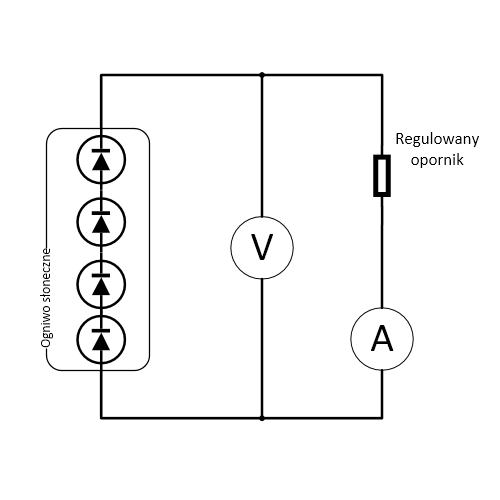
\includegraphics[width=1\textwidth]{img_fiz/Circuit}
  \caption{Obwód z ogniwem}
  \label{fig:sub1}
\end{subfigure}%
\begin{subfigure}{.5\textwidth}
  \centering
  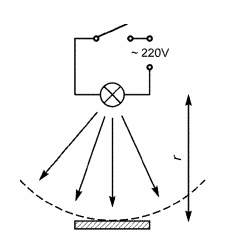
\includegraphics[width=1\textwidth]{img_fiz/Lamp}
  \caption{Lampa i ogniwo słoneczne}
  \label{fig:sub2}
\end{subfigure}
\caption{Układ doświadczalny}
\label{fig:test}
\end{figure}


\subsection{Wyniki pomiarów}

\begin{table}[H]
\centering
\caption{Natężenie światła}
\label{my-label}
\begin{tabular}{|p{3cm}|p{3cm}|}
\hline
$\phi$ {[}$W/m^2${]} & $\phi$ śr. {[}$W/m^2${]}\\
\hline
60,0	& 58,9   \\
65,2    &        \\
54,5    &        \\
55,8    &        \\
\hline   
\end{tabular}
\end{table}

\begin{table}[H]
\centering
\caption{Ogniwo polikrystaliczne - stałe}
\label{polistale}
\begin{tabular}{|p{2cm}|p{2cm}|p{2cm}|}
\hline
N & S {[}$cm^2${]} & N*S {[}$cm^2${]}   \\
\hline
8 & 7,8 & 62,4 \\
\hline
\end{tabular}
\end{table}

\begin{table}[H]
\centering
\caption{Ogniwo polikrystaliczne - pomiary}
\label{poliwyniki}
\begin{tabular}{|p{2cm}|p{2cm}|p{2cm}|p{2cm}|p{2cm}|}
\hline
I {[}$mA${]} & U {[}$V${]} & P  {[}$mW${]} & U/n {[}$V${]} & I/S {[}$A/m^2${]} \\
\hline
0,12 & 2,63 & 0,33 & 0,33 & 0,16 \\
0,17 & 2,62 & 0,44 & 0,33 & 0,22 \\
0,20 & 2,61 & 0,52 & 0,33 & 0,26 \\
0,60 & 2,53 & 1,52 & 0,32 & 0,77 \\
1,00 & 2,46 & 2,46 & 0,31 & 1,28 \\
1,43 & 2,37 & 3,39 & 0,30 & 1,83 \\
1,63 & 2,33 & 3,80 & 0,29 & 2,09 \\
1,85 & 2,28 & 4,22 & 0,29 & 2,37 \\
2,00 & 2,25 & 4,50 & 0,28 & 2,56 \\
2,24 & 2,18 & 4,88 & 0,27 & 2,87 \\
2,43 & 2,12 & 5,15 & 0,27 & 3,12 \\
2,69 & 2,05 & 5,51 & 0,26 & 3,45 \\
2,99 & 1,97 & 5,88 & 0,25 & 3,83 \\
3,22 & 1,89 & 6,09 & 0,24 & 4,13 \\
3,37 & 1,89 & 6,37 & 0,24 & 4,32 \\
3,55 & 1,74 & 6,16 & 0,22 & 4,55 \\
3,59 & 1,80 & 6,46 & 0,23 & 4,60 \\
3,87 & 1,52 & 5,86 & 0,19 & 4,96 \\
4,07 & 1,33 & 5,41 & 0,17 & 5,22 \\
4,25 & 1,11 & 4,71 & 0,14 & 5,45 \\
4,41 & 0,79 & 3,50 & 0,10 & 5,65 \\
4,51 & 0,67 & 3,03 & 0,08 & 5,78 \\
4,69 & 0,53 & 2,49 & 0,07 & 6,01\\
\hline
\end{tabular}
\end{table}

\newpage

\begin{table}[H]
\centering
\caption{Ogniwo monokrystaliczne - stałe}
\label{monostale}
\begin{tabular}{|p{2cm}|p{2cm}|p{2cm}|}
\hline
N & S {[}$cm^2${]} & N*S {[}$cm^2${]}   \\
\hline
1 & 63,0 & 63,0 \\
\hline
\end{tabular}
\end{table}

\begin{table}[H]
\centering
\caption{Ogniwo monokrystaliczne - pomiary}
\label{mono}
\begin{tabular}{|p{2cm}|p{2cm}|p{2cm}|p{2cm}|p{2cm}|}
\hline
I {[}$mA${]} & U {[}$V${]} & P  {[}$mW${]} & U/N {[}$V${]} & I/S {[}$A/m^2${]} \\ 
\hline
0,6 	& 0,46 & 0,27  & 0,46 & 0,10 \\
1       & 0,46 & 0,46  & 0,46 & 0,16 \\
1,7     & 0,46 & 0,78  & 0,46 & 0,27 \\
2,2     & 0,46 & 1,01  & 0,46 & 0,35 \\
3,6     & 0,46 & 1,64  & 0,46 & 0,57 \\
5,2     & 0,45 & 2,36  & 0,45 & 0,83 \\
7,1     & 0,45 & 3,21  & 0,45 & 1,13 \\
10,6    & 0,45 & 4,76  & 0,45 & 1,68 \\
15,7    & 0,44 & 6,96  & 0,44 & 2,49 \\
\hline
\end{tabular}
\end{table}


\begin{center}
\begin{tikzpicture}[scale=1.5]
\begin{axis}[
    title={Zależność gęstości prądu od napięcia na sekcję},
    xlabel={Napięcie na sekcję U/N [V]},
    ylabel={Gęstość prądu j [$A/m^2$]},
    xmin=0, xmax=0.5,
    ymin=0, ymax=8,
    xtick={0,0.1,0.2,0.3,0.4, 0.5},
    ytick={0,1,2,3,4,5,6,7, 8, 9},
    legend pos=north west,
    ymajorgrids=true,
    grid style=dashed,
]
 
\addplot[
    color=blue,
    mark=square,
    ]
    coordinates {
    (0.33,	0.16)
	(0.33,	0.22)
	(0.33,	0.26)
	(0.32,	0.77)
	(0.31,	1.28)
	(0.30,	1.83)
	(0.29,	2.09)
	(0.29,	2.37)
	(0.28,	2.56)
	(0.27,	2.87)
	(0.27,	3.12)
	(0.26,	3.45)
	(0.25,	3.83)
	(0.24,	4.13)
	(0.24,	4.32)
	(0.23,	4.60)	
	(0.22,	4.55)
	(0.19,	4.96)
	(0.17,	5.22)
	(0.14,	5.45)
	(0.10,	5.65)
	(0.08,	5.78)
	(0.07,	6.01)
    };
    \addlegendentry{Polikrystaliczne}
    
    \addplot[
    color=red,
    mark=square,
    ]
    coordinates {
    (0.46, 0.10)
	(0.46, 0.16)
	(0.46, 0.27)
	(0.46, 0.35)
	(0.46, 0.57)
	(0.45, 0.83)
	(0.45, 1.13)
	(0.45, 1.68)
	(0.44, 2.49)
    };
    \addlegendentry{Monokrystaliczne}
 
\end{axis}
\end{tikzpicture}
\end{center}

\newpage

\subsection{Omówienie wyników}
Pomiar napięcia i natężenia dla ogniwa polikrystalicznego dał o wiele ciekawszą krzywą, mówiącą więcej o ogólnym kształcie funkcji niż ogniwo monokrystaliczne, gdyż zakres oporu jakim dysponowaliśmy nie pozwolił na znaczne zmiany napięcia na tym ogniwie (różnica 0,02 V między napięciami na najmniejszym a największym możliwym oporze). Dlatego też choć maksymalna moc dla obu ogniw jest podobna, około 7 mW, można podejrzewać, że maksimum mocy dla ogniwa monokrystalicznego można zaobserwować dla oporu mniejszego niż najmniejszy dostępny przy oporniku, którym dysponowaliśmy. \\
W punkcie największej zmierzonej mocy ogniwo monokrystaliczne ma większe napięcie na sekcję, zaś ogniwo polikrystaliczne ma większą gęstość prądu.\\\\
Sprawność ogniwa wynosi 
$\eta = \dfrac{P}{P_{\text{źródła}}} = \dfrac{P}{\phi \times S}$ \\
zatem dla ogniwa:\\
polikrystalicznego 
$\eta = \dfrac{6,46 \times 10^{-3} W}{58,9 \frac{W}{m^2} \times 62,4 \times 10^{-4} m^2} \approx 1,76 \%$ \\\\
monokrystalicznego: 
$\eta = \dfrac{6,96 \times 10^{-3} W}{58,9 \frac{W}{m^2} \times 62,4 \times 10^{-4} m^2} \approx 1,89\% $  \\\\
Tak niska sprawność może wynikać np. z faktu, że ogniwo jest już stare i zużyte, może mieć też zanieczyszczoną powierzchnię, ponadto światło lampy mogło mieć niewłaściwą długość fali, przez co efekt fotowoltaiczny nie był odpowiednio wydajny.%

\subsection{Dyskusja błędu}
\begin{Huge}
DAWAJ ŁUKASZ
\end{Huge}
\end{document}